\documentclass[12pt,a4paper]{article}

% ==================== PACKAGES ====================
\usepackage[utf8]{inputenc}
\usepackage[T1]{fontenc}
\usepackage{helvet} % Cleaner, more modern font
\renewcommand{\familydefault}{\sfdefault}
\usepackage[margin=0.8in, top=1in, bottom=1in]{geometry}
\usepackage[table]{xcolor} % Added [table] for \rowcolor
\usepackage{hyperref}
\usepackage{graphicx}
\usepackage{booktabs}
\usepackage{longtable}
\usepackage{enumitem}
\usepackage{fancyhdr}
\usepackage{titlesec}
\usepackage{tcolorbox}
\usepackage{fontawesome5}
\usepackage{multicol}
\usepackage{tikz}
\usepackage{pgfplots}
\usepackage{array}
\usepackage{colortbl}
\usepackage{tabularx}
\usepackage{multirow}
\usepackage{wrapfig}
\usepackage{calc}
\pgfplotsset{compat=1.18}
\tcbuselibrary{skins, breakable, listings}
\usetikzlibrary{shadows, shapes, positioning, arrows.meta, calc}

% ==================== COLORS ====================
% Professional Blue Code Palette
\definecolor{primary}{RGB}{0, 78, 204}      % Vibrant Royal Blue
\definecolor{secondary}{RGB}{0, 40, 100}    % Deep Navy
\definecolor{accent}{RGB}{0, 180, 216}      % Cyan/Light Blue
\definecolor{success}{RGB}{46, 204, 113}    % Emerald Green
\definecolor{warning}{RGB}{241, 196, 15}    % Sunflower Yellow
\definecolor{danger}{RGB}{231, 76, 60}      % Alizarin Red
\definecolor{lightbg}{RGB}{240, 248, 255}   % Alice Blue
\definecolor{codebg}{RGB}{245, 245, 245}    % Light Gray
\definecolor{gold}{RGB}{255, 193, 7}        % Gold for highlights
\definecolor{purple}{RGB}{142, 68, 173}     % Purple for special elements
\definecolor{darkgray}{RGB}{52, 73, 94}     % Dark Gray for text

% ==================== HYPERREF SETUP ====================
\hypersetup{
    colorlinks=true,
    linkcolor=primary,
    urlcolor=primary,
    pdftitle={Data Structures & Algorithms with C++ - Mastery Course},
    pdfauthor={Mahmoud Salem},
    pdfsubject={DSA Course Syllabus 2026},
    pdfkeywords={DSA, C++, LeetCode, FAANG, Interview Prep}
}

% ==================== HEADER/FOOTER ====================
\setlength{\headheight}{25pt} % Increased headheight
\pagestyle{fancy}
\fancyhf{}
\fancyhead[L]{\textcolor{secondary}{\bfseries DSA Mastery}}
\fancyhead[R]{\textcolor{primary}{\bfseries Mahmoud Salem}}
\fancyfoot[L]{\footnotesize \faWhatsapp\ +20 101 162 0431}
\fancyfoot[R]{\footnotesize \faEnvelope\ ma7moudalysalem@gmail.com}
\fancyfoot[C]{\thepage}
\renewcommand{\headrulewidth}{1pt}
\renewcommand{\headrule}{\hbox to\headwidth{\color{primary}\leaders\hrule height \headrulewidth\hfill}}

% ==================== TITLE FORMATTING ====================
\titleformat{\section}
    {\Large\bfseries\color{secondary}}
    {\thesection}{1em}{\MakeUppercase}[\color{primary}\titlerule]
    
\titleformat{\subsection}
    {\large\bfseries\color{primary}}
    {\thesubsection}{1em}{}

% ==================== CUSTOM BOXES ====================
\newtcolorbox{featurebox}[1]{
    enhanced,
    colback=lightbg,
    colframe=primary,
    fonttitle=\bfseries\large,
    title={#1},
    rounded corners,
    drop shadow,
    boxrule=0.5mm,
    left=10pt, right=10pt, top=10pt, bottom=10pt
}

\newtcolorbox{importantbox}{
    enhanced,
    colback=red!5,
    colframe=danger,
    fonttitle=\bfseries,
    title={\faExclamationCircle\ Important Note},
    attach boxed title to top left={xshift=10pt, yshift*=-\tcboxedtitleheight/2},
    boxed title style={colback=danger}
}

\newtcolorbox{successbox}{
    enhanced,
    colback=green!5,
    colframe=success,
    fonttitle=\bfseries,
    title={\faCheckCircle\ Key Takeaway},
    attach boxed title to top left={xshift=10pt, yshift*=-\tcboxedtitleheight/2},
    boxed title style={colback=success}
}

\newtcolorbox{tipbox}{
    enhanced,
    colback=accent!10,
    colframe=accent,
    fonttitle=\bfseries,
    title={\faLightbulb\ Pro Tip},
    attach boxed title to top left={xshift=10pt, yshift*=-\tcboxedtitleheight/2},
    boxed title style={colback=accent}
}

\newtcolorbox{warningbox}{
    enhanced,
    colback=warning!10,
    colframe=warning,
    fonttitle=\bfseries,
    title={\faExclamationTriangle\ Important},
    attach boxed title to top left={xshift=10pt, yshift*=-\tcboxedtitleheight/2},
    boxed title style={colback=warning}
}

\newtcolorbox{quotebox}[1][]{
    enhanced,
    colback=lightbg,
    colframe=secondary,
    fonttitle=\bfseries\itshape,
    borderline west={4pt}{0pt}{primary},
    sharp corners,
    boxrule=0pt,
    left=15pt,
    #1
}

% ==================== DOCUMENT ====================
\begin{document}

% ==================== TITLE PAGE ====================
\begin{titlepage}
    \begin{tikzpicture}[remember picture, overlay]
        % Gradient background
        \fill[primary] (current page.north west) rectangle ([yshift=-5cm]current page.north east);
        \fill[secondary] ([yshift=-5cm]current page.north west) -- ([yshift=-8cm]current page.north east) -- ([yshift=-5cm]current page.north east) -- cycle;
        
        % Decorative circles
        \fill[accent, opacity=0.3] ([xshift=2cm, yshift=-3cm]current page.north west) circle (1.5cm);
        \fill[success, opacity=0.2] ([xshift=-3cm, yshift=-4cm]current page.north east) circle (2cm);
        
        \node[text=white, anchor=center, font=\fontsize{36}{40}\selectfont\bfseries] at ([yshift=-2.5cm]current page.north) {MASTER DATA STRUCTURES};
        \node[text=white, anchor=center, font=\fontsize{36}{40}\selectfont\bfseries] at ([yshift=-4cm]current page.north) {\& ALGORITHMS with C++ (C++17)};
    \end{tikzpicture}
    
    \vspace{5cm}
    \centering
    
    {\Large\bfseries\textcolor{secondary}{The Complete 7-Month Roadmap to Crack FAANG Interviews}}\\[0.5cm]
    {\large\textcolor{gray}{From Zero to Hero: Solve LeetCode Top 150 Interview Questions}}\\[1cm]
    
    \begin{tcolorbox}[colback=white, colframe=primary, width=14cm, enhanced, drop shadow, rounded corners]
        \centering
        \vspace{0.3cm}
        {\fontsize{24}{28}\selectfont\bfseries\textcolor{primary}{Starts: February 10, 2026}}\\[0.4cm]
        {\Large 56 Live Sessions \textcolor{primary}{|} Mentor Support \textcolor{primary}{|} Lifetime Access}\\[0.3cm]
        {\large\textcolor{gray}{Limited to 30 Students Only}}\\[0.2cm]
        \vspace{0.3cm}
    \end{tcolorbox}
    
    \vspace{1cm}
    
    \begin{multicols}{2}
        \begin{itemize}[label=\textcolor{success}{\faCheckCircle}, leftmargin=2cm, itemsep=8pt]
            \item \textbf{150+ LeetCode Problems}
            \item \textbf{Step-by-Step Visualizations}
            \item \textbf{Mock Interviews}
            \item \textbf{Resume Building \& Reviews}
            \item \textbf{Private Discord Community}
            \item \textbf{Certificate of Completion}
        \end{itemize}
    \end{multicols}
    
    \vspace{0.5cm}
    
    
\begin{tikzpicture}
        \node[fill=secondary, text=white, rounded corners=10pt, inner sep=18pt, drop shadow] {
            \fontsize{28}{32}\selectfont\bfseries ONLY \$150 USD
        };
    \end{tikzpicture}
    
    \vspace{0.8cm}
    
    \begin{tcolorbox}[colback=lightbg, colframe=primary, width=12cm, enhanced, rounded corners, boxrule=0.5mm]
        \centering
        {\large\bfseries\textcolor{secondary}{Instructor: Mahmoud Salem}}\\[0.2cm]
        {\normalsize Experienced Software Engineer \& Competitive Programmer}\\[0.1cm]
        {\small\textcolor{gray}{Google DSC Lead | 500+ LeetCode Problems Solved}}
    \end{tcolorbox}
    
    \vspace{0.8cm}
    
    \begin{tabular}{c c c}
        
\begin{tikzpicture}
            \node[fill=success, text=white, rounded corners=5pt, inner sep=8pt] {
                \faWhatsapp\ \textbf{+20 101 162 0431}
            };
        \end{tikzpicture} &
        \hspace{0.5cm} &
        
\begin{tikzpicture}
            \node[fill=primary, text=white, rounded corners=5pt, inner sep=8pt] {
                \faEnvelope\ \textbf{ma7moudalysalem@gmail.com}
            };
        \end{tikzpicture}
    \end{tabular}

\end{titlepage}

% ==================== COURSE INTRODUCTION ====================
\section{Welcome Message}

\begin{quotebox}
Welcome to the \textbf{Data Structures \& Algorithms with C++} course.

This course is designed to help you move from knowing how to write code to understanding how to \textit{think algorithmically}. You will learn how to analyze problems, break them down, and build correct and efficient solutions.

This is not a crash course. It is a \textbf{structured, long-term journey} that rewards consistency and effort.
\end{quotebox}

\vspace{0.5cm}

\section{Why This Course?}

\begin{featurebox}{\faRocket\ Accelerate Your Career}
This is not just another coding tutorial. It is a \textbf{comprehensive career transformation program}. Whether you are a student aiming for internships or a professional targeting top-tier tech companies, this course bridges the gap between theory and high-performance coding interviews. You will learn to \textit{think} like a software engineer, not just memorize solutions.
\end{featurebox}

\vspace{0.5cm}

\begin{quotebox}
\textit{``The goal is not to solve every problem. The goal is to recognize patterns so well that new problems feel familiar.''} \\[0.2cm]
\hfill --- \textbf{Mahmoud Salem}
\end{quotebox}

\vspace{0.5cm}

% ==================== WHAT YOU WILL GAIN ====================
\section{What You Will Gain}

\begin{center}
\begin{tcolorbox}[enhanced, colback=success!5, colframe=success, width=0.95\textwidth, rounded corners, drop shadow]
By the end of this course, you will be able to:
\begin{itemize}[label=\textcolor{success}{\faCheckCircle}, itemsep=8pt, leftmargin=1.5cm]
    \item Solve \textbf{150+ carefully selected LeetCode problems}
    \item Identify common algorithmic patterns instantly
    \item Master \textbf{recursion, trees, graphs, and dynamic programming}
    \item Analyze \textbf{time and space complexity} confidently
    \item Approach technical interviews with \textbf{clarity and confidence}
    \item Write \textbf{clean, optimized C++ code} using modern STL
    \item Communicate your thought process effectively during interviews
\end{itemize}
\end{tcolorbox}
\end{center}

\vspace{0.5cm}

\noindent
\begin{minipage}{0.48\textwidth}
    \subsection*{\faCode\ What You Will Master}
    \begin{itemize}[label=\textcolor{primary}{\faAngleRight}, itemsep=5pt]
        \item \textbf{Core DSA}: Arrays, Linked Lists, Trees, Graphs, DP.
        \item \textbf{C++ STL}: Power up your solutions with standard libraries.
        \item \textbf{Pattern Recognition}: Don't memorize; learn to \textit{see} the solution.
        \item \textbf{Time Complexity}: Analyze and optimize your code on the fly.
        \item \textbf{Interview Skills}: Communicate your thought process effectively.
    \end{itemize}
\end{minipage}
\hfill
\begin{minipage}{0.48\textwidth}
    \subsection*{\faUsers\ Who Is This For?}
    \begin{itemize}[label=\textcolor{primary}{\faUser}, itemsep=5pt]
        \item \textbf{Students}: CS undergrads preparing for placements.
        \item \textbf{Developers}: Looking to switch to product-based companies.
        \item \textbf{Career Changers}: Transitioning into software engineering.
        \item \textbf{Beginners}: Anyone willing to put in the hard work.
    \end{itemize}
\end{minipage}

\vspace{0.8cm}

% ==================== HOW THE COURSE IS STRUCTURED ====================
\section{How the Course Is Structured}

\begin{center}
\begin{tcolorbox}[enhanced, colback=lightbg, colframe=secondary, width=0.95\textwidth, rounded corners]
Each topic is delivered using a proven structure:
\begin{itemize}[label=\textcolor{primary}{\faAngleRight}, itemsep=10pt, leftmargin=1.5cm]
    \item \textbf{Concept Sessions} --- Intuition, mental models, visuals, and core ideas
    \item \textbf{Problem-Solving Sessions} --- Live solving of interview-level problems
    \item \textbf{Hybrid Sessions} --- Explanation combined with guided practice
    \item \textbf{Review Sessions} --- Consolidation and Q\&A at the end of each month
\end{itemize}
\vspace{0.3cm}
\textit{Special emphasis is placed on \textbf{recursion}, as it forms the foundation for trees, backtracking, and dynamic programming.}
\end{tcolorbox}
\end{center}

\vspace{0.5cm}

% ==================== STUDENT COMMITMENT ====================
\section{Student Commitment}

\begin{warningbox}
To benefit fully from this course, students are expected to:
\begin{itemize}[label=\textcolor{warning}{\faExclamationTriangle}, itemsep=6pt, leftmargin=1cm]
    \item Attend sessions regularly (\textbf{2 sessions per week})
    \item Review session material after each class
    \item Attempt problems \textbf{independently} before looking at solutions
    \item Accept struggle as part of the learning process
    \item Dedicate \textbf{1-2 hours daily} for practice
\end{itemize}
\vspace{0.3cm}
\centering
\textbf{\textit{Progress comes from consistency, not speed.}}
\end{warningbox}

% ==================== COURSE HIGHLIGHTS ====================
\section{Course Highlights}

\begin{center}
\begin{tikzpicture}[node distance=0.5cm]
    % Row 1
    \node[fill=primary, text=white, rounded corners=8pt, minimum width=4.5cm, minimum height=2cm, align=center, drop shadow] (n1) {\Large\faClock\\[0.2cm]\textbf{56 Live Sessions}};
    \node[fill=secondary, text=white, rounded corners=8pt, minimum width=4.5cm, minimum height=2cm, align=center, drop shadow, right=0.5cm of n1] (n2) {\Large\faCode\\[0.2cm]\textbf{150+ Problems}};
    \node[fill=accent, text=white, rounded corners=8pt, minimum width=4.5cm, minimum height=2cm, align=center, drop shadow, right=0.5cm of n2] (n3) {\Large\faCalendar\\[0.2cm]\textbf{7 Months}};
    
    % Row 2
    \node[fill=success, text=white, rounded corners=8pt, minimum width=4.5cm, minimum height=2cm, align=center, drop shadow, below=0.5cm of n1] (n4) {\Large\faVideo\\[0.2cm]\textbf{Session Recordings}};
    \node[fill=purple, text=white, rounded corners=8pt, minimum width=4.5cm, minimum height=2cm, align=center, drop shadow, right=0.5cm of n4] (n5) {\Large\faDiscord\\[0.2cm]\textbf{Discord Community}};
    \node[fill=danger, text=white, rounded corners=8pt, minimum width=4.5cm, minimum height=2cm, align=center, drop shadow, right=0.5cm of n5] (n6) {\Large\faCertificate\\[0.2cm]\textbf{Certificate}};
\end{tikzpicture}
\end{center}

\vspace{0.5cm}

\begin{tipbox}
\textbf{Session recordings} are available for 48 hours after each live session. Make sure to watch them if you miss a class!
\end{tipbox}

% ==================== CURRICULUM ====================
\newpage
\section{Comprehensive Curriculum Roadmap}

\begin{importantbox}
Each month includes \textbf{8 sessions} (2 per week). Sessions alternate between \textbf{Concept} lectures and \textbf{Problem-Solving} workshops. Total: \textbf{56 sessions} over 7 months.
\end{importantbox}

\vspace{0.5cm}

\begin{longtable}{|p{1.5cm}|p{4cm}|p{9.5cm}|}
\hline
\rowcolor{primary}
\textcolor{white}{\textbf{Month}} & \textcolor{white}{\textbf{Focus Area}} & \textcolor{white}{\textbf{Key Topics \& LeetCode Examples}} \\
\hline
\endfirsthead
\hline
\rowcolor{primary}
\textcolor{white}{\textbf{Month}} & \textcolor{white}{\textbf{Focus Area}} & \textcolor{white}{\textbf{Key Topics \& LeetCode Examples}} \\
\hline
\endhead

\textbf{Month 1} & \textbf{Foundations, Arrays \& Strings} & 
\begin{itemize}[leftmargin=*, nosep]
    \item Big-O Complexity, Memory Management, C++ STL Review
    \item Two Pointers, Sliding Window, Prefix Sum
    \item \textbf{Problems}: Two Sum, Best Time to Buy/Sell Stock, Maximum Subarray, Container With Most Water, 3Sum
\end{itemize} \\
\hline
\rowcolor{lightbg}
\textbf{Month 2} & \textbf{Linked Lists, Stacks \& Queues} & 
\begin{itemize}[leftmargin=*, nosep]
    \item Fast \& Slow Pointers, Monotonic Stack, Deque
    \item Cycle Detection, Merge Operations
    \item \textbf{Problems}: Reverse Linked List, Valid Parentheses, LRU Cache, Min Stack, Sliding Window Maximum
\end{itemize} \\
\hline
\textbf{Month 3} & \textbf{Recursion \& Backtracking} & 
\begin{itemize}[leftmargin=*, nosep]
    \item Call Stack Visualization, Base Cases, Pruning Techniques
    \item Decision Trees, State Space Trees
    \item \textbf{Problems}: Permutations, N-Queens, Subsets, Word Search, Combination Sum, Letter Combinations
\end{itemize} \\
\hline
\rowcolor{lightbg}
\textbf{Month 4} & \textbf{Trees \& Binary Search Trees} & 
\begin{itemize}[leftmargin=*, nosep]
    \item DFS (Preorder, Inorder, Postorder), BFS, Level-order
    \item Tree Properties, BST Operations, Tree Construction
    \item \textbf{Problems}: Max Depth, LCA, Validate BST, Serialize Tree, Binary Tree Paths, Invert Binary Tree
\end{itemize} \\
\hline
\textbf{Month 5} & \textbf{Heaps, Hashing \& Sorting} & 
\begin{itemize}[leftmargin=*, nosep]
    \item Priority Queues, Custom Comparators, Heap Operations
    \item Hash Maps, Hash Sets, Collision Handling
    \item \textbf{Problems}: Top K Frequent, Merge Intervals, Group Anagrams, Kth Largest Element, Meeting Rooms
\end{itemize} \\
\hline
\rowcolor{lightbg}
\textbf{Month 6} & \textbf{Graphs \& Binary Search} & 
\begin{itemize}[leftmargin=*, nosep]
    \item Graph Representations, BFS/DFS on Graphs
    \item Shortest Path (Dijkstra, BFS), Topological Sort, Union-Find
    \item Binary Search Variants, Search Space Reduction
    \item \textbf{Problems}: Number of Islands, Course Schedule, Clone Graph, Search in Rotated Array, Find Peak Element
\end{itemize} \\
\hline
\textbf{Month 7} & \textbf{Dynamic Programming \& Final Review} & 
\begin{itemize}[leftmargin=*, nosep]
    \item Memoization vs Tabulation, 1D/2D DP, State Transitions
    \item Classic DP Patterns: Knapsack, LIS, LCS, Grid DP
    \item \textbf{Problems}: Climbing Stairs, Coin Change, LCS, House Robber, Edit Distance, Unique Paths
\end{itemize} \\
\hline
\end{longtable}

% ==================== DETAILED SESSION BREAKDOWN ====================
\newpage
\section{Detailed Session Breakdown}

\subsection*{Month 1: Foundations, Arrays \& Strings (February 2026)}

\begin{center}
\begin{tabular}{|c|c|p{7cm}|p{4cm}|}
\hline
\rowcolor{secondary}
\textcolor{white}{\textbf{\#}} & \textcolor{white}{\textbf{Type}} & \textcolor{white}{\textbf{Topic}} & \textcolor{white}{\textbf{LeetCode}} \\
\hline
1 & Concept & Course Overview + C++ Review & -- \\
\hline
\rowcolor{lightbg}
2 & Concept & Time \& Space Complexity, STL Containers & -- \\
\hline
3 & Concept & Array Problem Patterns & -- \\
\hline
\rowcolor{lightbg}
4 & Solve & Two Pointers Technique & \#1, \#26, \#27, \#88 \\
\hline
5 & Concept & Sliding Window Technique & -- \\
\hline
\rowcolor{lightbg}
6 & Solve & Sliding Window Problems & \#121, \#209, \#643, \#3 \\
\hline
7 & Concept & Strings \& Character Handling & -- \\
\hline
\rowcolor{lightbg}
8 & Solve & String Problems & \#125, \#242, \#49, \#344 \\
\hline
\end{tabular}
\end{center}

\subsection*{Month 2: Linked Lists, Stack \& Queue (March 2026)}

\begin{center}
\begin{tabular}{|c|c|p{7cm}|p{4cm}|}
\hline
\rowcolor{secondary}
\textcolor{white}{\textbf{\#}} & \textcolor{white}{\textbf{Type}} & \textcolor{white}{\textbf{Topic}} & \textcolor{white}{\textbf{LeetCode}} \\
\hline
9 & Concept & Singly Linked Lists & -- \\
\hline
\rowcolor{lightbg}
10 & Solve & Linked List Problems & \#206, \#21, \#83, \#141 \\
\hline
11 & Concept & Fast \& Slow Pointer Technique & -- \\
\hline
\rowcolor{lightbg}
12 & Solve & Cycle / Middle Problems & \#142, \#876, \#234 \\
\hline
13 & Concept & Stack Fundamentals & -- \\
\hline
\rowcolor{lightbg}
14 & Solve & Stack Applications & \#20, \#155, \#496 \\
\hline
15 & Concept & Queue \& Deque & -- \\
\hline
\rowcolor{lightbg}
16 & Solve & Queue Problems & \#232, \#933, \#239 \\
\hline
\end{tabular}
\end{center}

\subsection*{Month 3: Recursion \& Backtracking (April 2026)}

\begin{warningbox}
This month is \textbf{intentionally extended} with extra practice sessions to ensure deep understanding of recursion concepts.
\end{warningbox}

\begin{center}
\begin{tabular}{|c|c|p{7cm}|p{4cm}|}
\hline
\rowcolor{secondary}
\textcolor{white}{\textbf{\#}} & \textcolor{white}{\textbf{Type}} & \textcolor{white}{\textbf{Topic}} & \textcolor{white}{\textbf{LeetCode}} \\
\hline
17 & Concept & Introduction to Recursion & -- \\
\hline
\rowcolor{lightbg}
18 & Concept & Call Stack and Base Cases & -- \\
\hline
19 & Hybrid & Recursion on Arrays & \#509, \#70 \\
\hline
\rowcolor{lightbg}
20 & Solve & Recursion Practice & \#344, \#206 \\
\hline
21 & Concept & Backtracking Fundamentals & -- \\
\hline
\rowcolor{lightbg}
22 & Solve & Backtracking Problems & \#46, \#78, \#77 \\
\hline
23 & Hybrid & Recursion Tree Analysis & \#22, \#17 \\
\hline
\rowcolor{lightbg}
24 & Review & Full Recursion Review & Mixed \\
\hline
\end{tabular}
\end{center}

\subsection*{Month 4: Trees \& Binary Search Trees (May 2026)}

\begin{center}
\begin{tabular}{|c|c|p{7cm}|p{4cm}|}
\hline
\rowcolor{secondary}
\textcolor{white}{\textbf{\#}} & \textcolor{white}{\textbf{Type}} & \textcolor{white}{\textbf{Topic}} & \textcolor{white}{\textbf{LeetCode}} \\
\hline
25 & Concept & Binary Tree Fundamentals & -- \\
\hline
\rowcolor{lightbg}
26 & Solve & DFS Traversals & \#94, \#144, \#145 \\
\hline
27 & Concept & BFS / Level Order Traversal & -- \\
\hline
\rowcolor{lightbg}
28 & Solve & BFS Problems & \#102, \#199 \\
\hline
29 & Concept & Tree Properties & -- \\
\hline
\rowcolor{lightbg}
30 & Solve & Height / Diameter & \#104, \#543 \\
\hline
31 & Concept & Binary Search Trees & -- \\
\hline
\rowcolor{lightbg}
32 & Solve & BST Problems & \#98, \#230, \#235 \\
\hline
\end{tabular}
\end{center}

\subsection*{Month 5: Heap, Hashing \& Sorting (June 2026)}

\begin{center}
\begin{tabular}{|c|c|p{7cm}|p{4cm}|}
\hline
\rowcolor{secondary}
\textcolor{white}{\textbf{\#}} & \textcolor{white}{\textbf{Type}} & \textcolor{white}{\textbf{Topic}} & \textcolor{white}{\textbf{LeetCode}} \\
\hline
33 & Concept & Heap and Priority Queue & -- \\
\hline
\rowcolor{lightbg}
34 & Solve & Heap Problems & \#215, \#347, \#295 \\
\hline
35 & Concept & Hash Tables & -- \\
\hline
\rowcolor{lightbg}
36 & Solve & Hashing Problems & \#1, \#217, \#451 \\
\hline
37 & Concept & Sorting Algorithms & -- \\
\hline
\rowcolor{lightbg}
38 & Solve & Sorting Problems & \#912, \#56, \#57 \\
\hline
39 & Hybrid & Custom Sorting / Comparators & \#179, \#75 \\
\hline
\rowcolor{lightbg}
40 & Review & Monthly Review & Mixed \\
\hline
\end{tabular}
\end{center}

\newpage

\subsection*{Month 6: Binary Search \& Graphs (July 2026)}

\begin{center}
\begin{tabular}{|c|c|p{7cm}|p{4cm}|}
\hline
\rowcolor{secondary}
\textcolor{white}{\textbf{\#}} & \textcolor{white}{\textbf{Type}} & \textcolor{white}{\textbf{Topic}} & \textcolor{white}{\textbf{LeetCode}} \\
\hline
41 & Concept & Binary Search Fundamentals & -- \\
\hline
\rowcolor{lightbg}
42 & Solve & Binary Search Problems & \#704, \#33, \#34 \\
\hline
43 & Concept & Graph Representation (Adj List/Matrix) & -- \\
\hline
\rowcolor{lightbg}
44 & Solve & DFS / BFS on Graphs & \#200, \#133, \#417 \\
\hline
45 & Concept & Topological Sorting & -- \\
\hline
\rowcolor{lightbg}
46 & Solve & Topological Problems & \#207, \#210, \#269 \\
\hline
47 & Hybrid & Grid Graph Problems & \#695, \#994, \#286 \\
\hline
\rowcolor{lightbg}
48 & Review & Graph Review & Mixed \\
\hline
\end{tabular}
\end{center}

\subsection*{Month 7: Dynamic Programming \& Final Revision (August 2026)}

\begin{successbox}
This is the \textbf{culmination} of everything you've learned. DP builds on recursion, trees, and pattern recognition. Stay focused!
\end{successbox}

\begin{center}
\begin{tabular}{|c|c|p{7cm}|p{4cm}|}
\hline
\rowcolor{secondary}
\textcolor{white}{\textbf{\#}} & \textcolor{white}{\textbf{Type}} & \textcolor{white}{\textbf{Topic}} & \textcolor{white}{\textbf{LeetCode}} \\
\hline
49 & Concept & Dynamic Programming Introduction & -- \\
\hline
\rowcolor{lightbg}
50 & Solve & 1D Dynamic Programming & \#70, \#198, \#213 \\
\hline
51 & Concept & Knapsack Pattern & -- \\
\hline
\rowcolor{lightbg}
52 & Solve & Knapsack Problems & \#416, \#494, \#322 \\
\hline
53 & Concept & LIS and LCS Patterns & -- \\
\hline
\rowcolor{lightbg}
54 & Solve & LIS / LCS Problems & \#300, \#1143, \#72 \\
\hline
55 & Solve & Advanced DP (Grid / 2D) & \#62, \#64, \#221 \\
\hline
\rowcolor{lightbg}
56 & Final & \textbf{Full Course Revision} & Top 150 \\
\hline
\end{tabular}
\end{center}

% ==================== PROBLEM SOLVING PATTERNS ====================
\newpage
\section{Problem-Solving Patterns You Will Master}

\begin{center}
\begin{tikzpicture}
    % Pattern boxes
    \node[fill=primary, text=white, rounded corners=5pt, minimum width=4cm, minimum height=1.2cm, align=center] (p1) at (0,0) {\textbf{Two Pointers}};
    \node[fill=secondary, text=white, rounded corners=5pt, minimum width=4cm, minimum height=1.2cm, align=center] (p2) at (5,0) {\textbf{Sliding Window}};
    \node[fill=accent, text=white, rounded corners=5pt, minimum width=4cm, minimum height=1.2cm, align=center] (p3) at (10,0) {\textbf{Fast \& Slow}};
    
    \node[fill=success, text=white, rounded corners=5pt, minimum width=4cm, minimum height=1.2cm, align=center] (p4) at (0,-1.8) {\textbf{Binary Search}};
    \node[fill=purple, text=white, rounded corners=5pt, minimum width=4cm, minimum height=1.2cm, align=center] (p5) at (5,-1.8) {\textbf{BFS / DFS}};
    \node[fill=danger, text=white, rounded corners=5pt, minimum width=4cm, minimum height=1.2cm, align=center] (p6) at (10,-1.8) {\textbf{Backtracking}};
    
    \node[fill=warning, text=black, rounded corners=5pt, minimum width=4cm, minimum height=1.2cm, align=center] (p7) at (0,-3.6) {\textbf{Monotonic Stack}};
    \node[fill=darkgray, text=white, rounded corners=5pt, minimum width=4cm, minimum height=1.2cm, align=center] (p8) at (5,-3.6) {\textbf{Union-Find}};
    \node[fill=primary!70, text=white, rounded corners=5pt, minimum width=4cm, minimum height=1.2cm, align=center] (p9) at (10,-3.6) {\textbf{Dynamic Programming}};
\end{tikzpicture}
\end{center}

\vspace{0.5cm}

\begin{successbox}
Mastering these \textbf{9 core patterns} will allow you to solve \textbf{90\%+} of coding interview questions!
\end{successbox}

% ==================== PREREQUISITES ====================
\section{Prerequisites}

\begin{center}
\begin{tcolorbox}[enhanced, colback=lightbg, colframe=secondary, width=0.9\textwidth, rounded corners]
\begin{multicols}{2}
    \begin{itemize}[label=\textcolor{success}{\faCheck}, itemsep=8pt]
        \item Basic understanding of any programming language
        \item Familiarity with C++ syntax (variables, loops, functions)
        \item A computer with stable internet connection
        \item Dedication to practice \textbf{1-2 hours daily}
    \end{itemize}
    \columnbreak
    \begin{itemize}[label=\textcolor{danger}{\faTimes}, itemsep=8pt]
        \item No prior DSA knowledge required
        \item No competitive programming experience needed
        \item No computer science degree required
        \item No previous interview experience needed
    \end{itemize}
\end{multicols}
\end{tcolorbox}
\end{center}

\begin{tipbox}
Basic familiarity with C++ is enough. The course includes a \textbf{focused C++ review} session tailored specifically for problem solving in the first week!
\end{tipbox}

% ==================== FAQ ====================
\newpage
\section{Frequently Asked Questions}

\begin{featurebox}{\faQuestionCircle\ Is this course suitable for beginners?}
\textbf{Yes!} The course is designed for committed learners. Difficulty increases gradually with continuous support. We start from the basics and build up systematically.
\end{featurebox}

\vspace{0.3cm}

\begin{featurebox}{\faQuestionCircle\ Will we really solve all LeetCode Top 150 problems?}
\textbf{Absolutely.} The course roadmap is meticulously designed to cover the entire LeetCode Top 150 Interview Questions list, plus additional problems for practice.
\end{featurebox}

\vspace{0.3cm}

\begin{featurebox}{\faQuestionCircle\ What if I miss a live session?}
All sessions are \textbf{recorded} and available for \textbf{48 hours} after the live session. You can catch up and ask questions in the Discord community.
\end{featurebox}

\vspace{0.3cm}

\begin{featurebox}{\faQuestionCircle\ What if I struggle with problems?}
Struggling is \textbf{expected and encouraged!} It is a necessary part of building problem-solving skills. The Discord community and weekly Q\&A sessions are here to help.
\end{featurebox}

\vspace{0.3cm}

\begin{featurebox}{\faQuestionCircle\ Will I get a certificate?}
\textbf{Yes!} Upon successful completion of the course and assignments, you will receive an official \textbf{Certificate of Completion} that you can add to your LinkedIn profile.
\end{featurebox}

\vspace{0.3cm}

\begin{featurebox}{\faQuestionCircle\ What is the refund policy?}
We offer a \textbf{7-day money-back guarantee}. If you're not satisfied after the first week, you can request a full refund --- no questions asked.
\end{featurebox}

% ==================== ENROLLMENT ====================
\newpage
\section{Enrollment \& Investment}

\begin{center}
    \begin{tcolorbox}[enhanced, colback=white, colframe=secondary, width=0.95\textwidth, drop shadow, rounded corners, boxrule=1mm]
        \centering
        \vspace{0.3cm}
        {\fontsize{22}{26}\selectfont\bfseries \faGraduationCap\ Ready to Transform Your Career?}\\[0.6cm]
        
        This course is an investment in your future. The skills you gain here are the same ones used by engineers at \textbf{Google}, \textbf{Meta}, \textbf{Amazon}, \textbf{Microsoft}, and \textbf{Apple}.\\[0.6cm]
        
        
\begin{tikzpicture}
            \node[fill=secondary, text=white, rounded corners=15pt, inner sep=20pt, drop shadow] {
                \fontsize{36}{40}\selectfont\bfseries \$150 USD
            };
        \end{tikzpicture}
        
        \vspace{0.5cm}
        {\large\textcolor{gray}{One-Time Payment | No Hidden Fees | Lifetime Value}}
        
        \vspace{0.6cm}
        
        \begin{tabular}{rl rl}
            \Large\faCalendarCheck & \Large\textbf{Start Date:} February 10, 2026 &
            \Large\faClock & \Large\textbf{Duration:} 7 Months \\[0.4cm]
            \Large\faUsers & \Large\textbf{Class Size:} Max 30 Students &
            \Large\faVideo & \Large\textbf{Sessions:} 56 Live Classes \\[0.4cm]
            \Large\faDiscord & \Large\textbf{Community:} Private Discord &
            \Large\faCertificate & \Large\textbf{Certificate:} Upon Completion \\
        \end{tabular}
        
        \vspace{0.8cm}
        
        \begin{tcolorbox}[enhanced, colback=success!10, colframe=success, width=0.85\textwidth, rounded corners]
            \centering
            {\large\bfseries\textcolor{success}{\faCheckCircle\ 7-Day Money-Back Guarantee}}\\[0.2cm]
            {\normalsize Not satisfied after the first week? Get a full refund, no questions asked.}
        \end{tcolorbox}
        
        \vspace{0.6cm}
        {\Large\bfseries Reserve Your Spot Today:}\\[0.4cm]
        
        \begin{tikzpicture}
            \node[fill=success, text=white, rounded corners=8pt, inner sep=15pt, drop shadow] {
                \Large\bfseries \faWhatsapp\ +20 101 162 0431
            };
        \end{tikzpicture}
        \hspace{1cm}
        
\begin{tikzpicture}
            \node[fill=primary, text=white, rounded corners=8pt, inner sep=15pt, drop shadow] {
                \Large\bfseries \faEnvelope\ ma7moudalysalem@gmail.com
            };
        \end{tikzpicture}
        \vspace{0.4cm}
    \end{tcolorbox}
\end{center}

\vspace{0.5cm}

\begin{quotebox}
\textit{``This course is designed for students who want \textbf{real improvement}, not shortcuts. If you stay \textbf{consistent} and \textbf{trust the process}, your problem-solving skills will improve \textbf{dramatically}.''}\\[0.2cm]
\hfill --- \textbf{Mahmoud Salem}
\end{quotebox}

% ==================== INSTRUCTOR ====================
\section{About Your Instructor}

\begin{center}
\begin{tcolorbox}[enhanced, colback=lightbg, colframe=primary, width=0.9\textwidth, rounded corners, drop shadow]
    \centering
    \vspace{0.3cm}
    {\fontsize{20}{24}\selectfont\bfseries\textcolor{secondary}{Mahmoud Salem}}\\[0.3cm]
    {\large\textit{Software Engineer \& Competitive Programmer}}\\[0.5cm]
    
    \begin{multicols}{2}
        \begin{itemize}[label=\textcolor{primary}{\faAngleRight}, itemsep=5pt, leftmargin=1cm]
            \item 500+ LeetCode Problems Solved
            \item Former Google DSC Lead
            \item 4+ Years of Teaching Experience
            \item Multiple Hackathon Winner
        \end{itemize}
        \columnbreak
        \begin{itemize}[label=\textcolor{primary}{\faAngleRight}, itemsep=5pt, leftmargin=1cm]
            \item Mentored 200+ Students
            \item Expert in C++ and Python
            \item Active Open Source Contributor
            \item Published Technical Writer
        \end{itemize}
    \end{multicols}
    \vspace{0.3cm}
\end{tcolorbox}
\end{center}

% ==================== FINAL CTA ====================
\vspace{0.5cm}

\begin{center}

\begin{tikzpicture}
    \node[fill=primary, text=white, rounded corners=10pt, inner sep=20pt, drop shadow, minimum width=14cm] {
        \begin{minipage}{13cm}
            \centering
            {\Large\bfseries \faRocket\ Don't Wait --- Start Your Journey Today!}\\[0.3cm]
            {\normalsize Limited to 30 students. Secure your spot before it's too late.}\\[0.3cm]
            {\large\faWhatsapp\ \textbf{+20 101 162 0431} \hspace{1cm} \faEnvelope\ \textbf{ma7moudalysalem@gmail.com}}
        \end{minipage}
    };
\end{tikzpicture}
\end{center}

\end{document}
